\documentclass[11pt,a4paper]{article}

\usepackage[T1]{fontenc}
\usepackage[utf8]{inputenc}
\usepackage{lmodern}
\usepackage[margin=2.5cm]{geometry}
\usepackage{microtype}
\usepackage{amsmath,amssymb,amsthm}
\usepackage{booktabs}
\usepackage{tabularx}
\usepackage{array}
\usepackage{enumitem}
\usepackage{xcolor}
\usepackage{textcomp}
\usepackage{listings}
\usepackage{tikz}
\usetikzlibrary{arrows.meta,positioning}
\usepackage[font=small,labelfont=bf]{caption}
\usepackage[round,authoryear]{natbib}
\usepackage[colorlinks=true,linkcolor=black,citecolor=blue!50!black,urlcolor=blue!50!black]{hyperref}

% ---- theorem environments -------------------------------------------------
\theoremstyle{definition}
\newtheorem{definition}{Definition}
\newtheorem{assumption}{Assumption}
\newtheorem{prediction}{Prediction}
\theoremstyle{plain}
\newtheorem{proposition}{Proposition}
\newtheorem{corollary}{Corollary}
\theoremstyle{remark}
\newtheorem{remark}{Remark}

% ---- Lean listings ----------------------------------------------------------
\lstdefinestyle{lean}{
  basicstyle=\ttfamily\fontsize{7.7}{9.5}\selectfont,
  showlines=true,
  upquote=true,
  columns=fullflexible,
  keepspaces=true,
  breaklines=true,
  showstringspaces=false,
  frame=single,
  framerule=0.3pt,
  rulecolor=\color{black!35},
  xleftmargin=3pt,
  xrightmargin=3pt,
  aboveskip=8pt,
  belowskip=8pt,
  literate=
    {ℕ}{{$\mathbb{N}$}}1 {ℤ}{{$\mathbb{Z}$}}1 {↑}{{$\uparrow$}}1
    {→}{{$\to$}}1 {←}{{$\leftarrow$}}1 {↔}{{$\leftrightarrow$}}1
    {∀}{{$\forall$}}1 {∃}{{$\exists$}}1 {¬}{{$\neg$}}1 {∧}{{$\land$}}1
    {≠}{{$\neq$}}1 {≤}{{$\leq$}}1 {≡}{{$\equiv$}}1
    {₁}{{$_1$}}1 {₂}{{$_2$}}1
    {Σ}{{$\Sigma$}}1 {Δ}{{$\Delta$}}1 {φ}{{$\varphi$}}1 {σ}{{$\sigma$}}1
    {⟨}{{$\langle$}}1 {⟩}{{$\rangle$}}1
    {§}{{\S}}1 {–}{{--}}1 {—}{{---}}1 {·}{{\textbullet}}1
}
\lstset{style=lean}

% ---- small macros -----------------------------------------------------------
\newcommand{\N}{\mathbb{N}}
\newcommand{\Z}{\mathbb{Z}}
\newcommand{\Dt}{\Delta t}
\newcommand{\code}[1]{\texttt{#1}}
\newcommand{\produce}{\mathit{produce}}
\newcommand{\valid}{\mathit{valid}}
\newcommand{\faithful}{\mathit{faithful}}

\setlist{itemsep=2pt,topsep=4pt}
\renewcommand{\arraystretch}{1.25}
\newcolumntype{L}{>{\raggedright\arraybackslash}X}
\newcolumntype{P}[1]{>{\raggedright\arraybackslash}p{#1}}

\hypersetup{
  pdftitle={Typed Crossings: What Casts, Refinement Proofs and Chain-of-Thought Checks Carry Across a Boundary},
  pdfauthor={Bernhard Kreinz},
  pdfkeywords={coercions, refinement, hyperproperties, chain-of-thought faithfulness, proof assistants, Lean 4, typed edges, layered models}
}

\begin{document}

\begin{center}
  {\LARGE\bfseries Typed Crossings\par}
  \vspace{0.5em}
  {\large What Casts, Refinement Proofs and Chain-of-Thought Checks\\
   Carry Across a Boundary\par}
  \vspace{1.4em}
  {\large Bernhard Kreinz\par}
  \vspace{0.3em}
  {\normalsize Barnes Projects\par}
  {\small ORCID: \href{https://orcid.org/0009-0005-2148-9903}{0009-0005-2148-9903}\par}
  \vspace{0.8em}
  {\small Version 1.0 (preprint) \textperiodcentered{} November 2026 \textperiodcentered{}
   DOI: \href{https://doi.org/10.5281/zenodo.24219769}{10.5281/zenodo.24219769}\par}
\end{center}

\vspace{0.6em}

\begin{abstract}
\noindent
A claim established in one structure is routinely reused in another: an identity on the
natural numbers after a cast to the integers, a property of a specification after
refinement to an implementation, the validity of a written chain of reasoning as a
statement about the computation that produced it. Whether the claim survives is a property
of the map that carries it, and it cannot be read off the symbol or the word that is
reused. This position paper argues that such a crossing should be declared and typed: by
its \emph{kind}, which fixes what a failure of the crossing consists in, and by what it
\emph{preserves}, under which conditions. Three cases are examined. In Lean~4, Mathlib's
bundled morphisms and cast lemmas type the crossing wherever cast automation works. In
system verification, properties beyond functional correctness are carried across a
refinement one preservation proof at a time. In machine learning, the validity of a
model's written reasoning and its faithfulness to the model's computation are two
different crossings. A judgement on the trace alone can agree with faithfulness exactly
when faithfulness does not vary among the computations that write the same trace; where
one trace is written by two computations and describes only one of them, no check on the
trace tells the two apart. Verify the trace, and you have verified the trace. Each field
already handles the problem locally. The contribution is a common vocabulary, taken from
Layered Event Modelling, that states what the local solutions share, together with a
Lean~4 mechanisation: the underlying graph model, a crossing with a declared kind and
associated preservation proofs, with casts as the worked example, and the results on
traces. The
mechanised results are elementary, the mechanisation covers only part of the paper, no
new experiments are reported, and the paper states where its claims stop.
\end{abstract}

\noindent\textbf{Keywords:} coercions; refinement; hyperproperties; chain-of-thought
faithfulness; proof assistants; Lean~4; typed edges; layered models.

\vspace{0.8em}

\section{Introduction}
\label{sec:intro}

Three problems from three fields have the same shape.

\paragraph{A cast.} In the proof assistant Lean~4 \citep{demoura2021}, the two expressions
below differ only in where a natural number is turned into an integer. The first evaluates
to $0$, the second to $-1$:
\begin{lstlisting}
example : ((2 - 3 : Nat) : Int) = 0 := rfl
example : ((2 : Nat) - (3 : Nat) : Int) = -1 := rfl
\end{lstlisting}
The symbol \code{-} is the same in both lines. What it means depends on which side of the
cast it is evaluated on, and the author of the expression does not write the cast.

\paragraph{A verified kernel.} The functional-correctness proof of the seL4 microkernel
establishes that its C implementation refines an abstract specification
\citep{klein2009}. The proof has no notion of time and so makes no claim about timing
channels. Isolation in time had to be added later, as a mechanism of its own
\citep{ge2019}. The kernel was verified, and a property a user might take ``verified'' to
include was not among the properties the proof carried from the specification to the
code.

\paragraph{A valid chain of reasoning.} A language model writes out a chain of steps
before its answer, or a proof that a proof checker accepts. A check on that text can
establish that every step follows from the ones before it. It does not establish that the
text describes how the model arrived at its answer. In controlled studies, models whose
answers were changed by a hint often did not mention the hint in the reasoning they wrote
\citep{turpin2023,chen2025}.

\medskip
In each case a claim is established on one side of a boundary and reused on the other: an
identity on $\N$ reused on $\Z$, a property of a specification reused of an
implementation, the validity of a text reused as an account of a computation. Whether the
reuse is sound depends on the map or relation that crosses the boundary, on what kind of
crossing it is and on what it preserves. In each case the thing that is reused, a symbol,
the word ``verified'', the word ``reasoning'', does not say.

\paragraph{Thesis.} A crossing along which claims are carried should be declared and
typed: by its kind, which fixes what a failure of the crossing consists in, and by what it
preserves, under which conditions.

\paragraph{What the fields already do.} None of the three fields lacks this insight. Each
applies it locally. Lean's mathematical library Mathlib records what a cast preserves in
bundled morphisms and in lemmas registered for its cast tactics
\citep{mathlib2020,lewis2020}. Verification practice proves the preservation of each
further property separately, and the theory of secure compilation classifies compilers by
the class of properties they preserve \citep{clarkson2010,abate2019}. Interpretability
research separates the faithfulness of an explanation from its plausibility and tests the
former by intervening on the model \citep{jacovi2020,geiger2025}. What these local
solutions have in common is not usually stated, because the three literatures do not
share a vocabulary. This paper proposes one.

\paragraph{Kind of paper.} This is a position paper with a machine-checked artefact. It
reports no new experiments and proves no deep theorem. Its claims are of three sorts:
readings of existing practice, which can be checked against the literature cited;
definitions and elementary results, some of which are checked in Lean; and two
predictions, which are marked as untested.

\paragraph{Contributions.}
\begin{enumerate}[label=(\arabic*)]
  \item \emph{A common reading of three practices.} Cast lemmas in Mathlib, per-property
        preservation proofs in system verification, and faithfulness tests for written
        model reasoning are shown to address one situation: a claim established on one
        side of a crossing is reused on the other
        (Sections~\ref{sec:casts}--\ref{sec:reasoning}).
  \item \emph{A small vocabulary for declaring a crossing.} A crossing is declared by its
        kind and by what it preserves (Section~\ref{sec:rule}). The kind cannot be
        inferred from the map alone, because two maps with the same formal properties can
        differ in the role in which they are used (Section~\ref{sec:three-kinds}). The
        vocabulary is taken from Layered Event Modelling \citep{kreinzlem} and restated
        here in the minimal form the argument needs.
  \item \emph{What a check on a trace certifies.} The validity of a written trace and its
        faithfulness to the computation that produced it are crossings of different
        kinds. A judgement made on the trace alone can agree with faithfulness exactly
        when faithfulness does not vary among the computations that write the same
        trace. Where one trace is written by two computations and describes only one of
        them, no such judgement exists (Section~\ref{sec:kernel}).
  \item \emph{A partial mechanisation.} The graph model behind the vocabulary, the
        typed crossing with two worked examples from the first case, and the results on
        traces are formalised in Lean~4 and published as an open-source package
        \citep{kreinzlemlean}. The refinement case is not formalised.
        Section~\ref{sec:mech} states what the mechanisation does and does not
        establish.
  \item \emph{Two testable predictions} about where automated provers fail and about
        what a declaration of kind adds
        (Section~\ref{sec:limits}).
\end{enumerate}

\paragraph{What is not claimed.} The paper does not claim that any of the three fields
has overlooked the problem; that the vocabulary of Layered Event Modelling transfers to
other domains in general, since three cases chosen by the author are evidence and not
proof; that written model reasoning is usually unfaithful, or of no value as evidence; or
that checking the results in Lean shows the definitions to fit real systems.

\paragraph{Outline.} Section~\ref{sec:rule} states the rule and the vocabulary.
Sections~\ref{sec:casts}, \ref{sec:refinement} and~\ref{sec:reasoning} are the three
cases; each is written to be read without the others and without background in the other
fields. Section~\ref{sec:mech} describes the mechanisation, Section~\ref{sec:related} the
related work, and Section~\ref{sec:limits} the limitations and the predictions.

\section{Typed crossings}
\label{sec:rule}

\subsection{The argument}
\label{sec:argument}

Mathematicians apply a single symbol or predicate, such as $+$, $\le$, $\cong$,
\emph{compact} or \emph{valid}, to objects of quite different construction. On the
blackboard this abuse of notation is a feature. It compresses the exposition, because a
competent reader reconstructs which structure is meant. A proof assistant has no such
reader, and neither has the formal verification of a compiler or a kernel, nor the
evaluation of a model's output. There the following argument applies.

\begin{enumerate}[label=(P\arabic*)]
  \item Distinct structures may give one symbol different truth conditions. Subtraction
        on the natural numbers is not subtraction on the integers.
  \item Reusing the symbol is harmless where its truth conditions are invariant under the
        map between the structures. Where they are not, the reuse conceals a shift.
  \item Which of the two holds is a property of the map and the operation together. It
        cannot be read off the symbol.
  \item Where the properties of the map are not declared, every proof and every claim
        that crosses the boundary must establish them again, case by case. Where they are
        declared, the crossing can be automated and its failure conditions can be stated.
\end{enumerate}

\noindent
(P1)--(P3) are uncontroversial. (P4) is the practical premise, and the three cases are
offered as evidence for it.

\subsection{Vocabulary}
\label{sec:vocabulary}

The vocabulary is taken from Layered Event Modelling (LEM; \citealp{kreinzlem}), a method
proposal for layered models of cyber and operational risk. LEM's axioms are stipulations
adopted for their consequences, not theorems, and LEM says of itself that its transfer to
other domains is untested and would have to be argued, not read off a resemblance. The
cases below are such an argument for three domains. Only the following elements are
used.

\paragraph{Layers and locality.} A model assigns every node to exactly one layer (node
typing, LEM axiom A1). A predicate is defined at a declared layer and may be reused at
another only where its truth conditions and argument structure are demonstrably invariant
(predicate locality, A2). Where nodes of different layers refer to the same thing, that
co-reference is declared as a relation between distinct nodes (A3), so that a claim about
one is not silently transferred to the other.

\paragraph{Typed edges.} Every edge carries a declared type (A4). LEM types edges by what
would have to be true for the edge to fail, and distinguishes six types
(Table~\ref{tab:edges}). The table separates two things that the word ``fail'' can cover.
An edge does not hold when what it asserts is false under fixed conditions. An edge can
also depend on something declared, a scheme, a norm, a convention or a set of
assumptions, and can then cease to hold while the world stays as it is, because what
was declared is changed. That is a change of the conditions under which the edge is
judged, not an error in judging it. LEM uses this dependence as a test for
classificatory and normative edges. The table does not treat it as exclusive to them.
The type determines which properties are defined for the edge.
Duration, written $\Dt$, is defined for causal edges only: it is the duration of a
transition along which one event brings about the next. For every other type it is
undefined, not zero. The type of an edge is decided per edge, by test, and not by which
pair of layers the edge connects. Two of LEM's tests are used below: whether a non-zero
interval between the two ends is coherent, and whether an intervention can break the edge
without changing what its two ends are \citep{woodward2003}.

\begin{table}[t]
\centering\small
\begin{tabularx}{\textwidth}{@{}P{2.7cm}LLP{3.0cm}c@{}}
\toprule
Edge type & What the edge asserts & Does not hold when &
  Ceases to hold, the world unchanged, when & $\Dt$ \\
\midrule
Causal & One event brings about another, under intervention. &
  The transition does not occur, or is interrupted. & --- & defined \\
Constitutive & One state realises another at the same time; nothing propagates. &
  The realising states do not obtain. & --- & --- \\
Classificatory & An object satisfies the criteria of a declared scheme. &
  The criteria are not met. & The scheme is changed. & --- \\
Normative & An act or omission stands as fulfilment, or as violation, of a norm. &
  The asserted standing is wrong under the applicable norm. &
  The norm is amended, or no longer applies to the case. & --- \\
Representational & A representation corresponds to a referent. &
  The representation does not correspond (misrepresentation). &
  The convention under which it is read is changed. & --- \\
Evidential & An observation supports an inference. &
  The observation does not support the inference. &
  The background assumptions are changed. & --- \\
\bottomrule
\end{tabularx}
\caption{The six edge types of LEM, restated. The third column gives what makes the
asserted relation false under fixed conditions. The fourth gives what the edge depends
on that is declared and could be changed. The entries for the last two rows are this
paper's reading, not LEM's. Duration is defined for causal edges only.}
\label{tab:edges}
\end{table}

\paragraph{Five structures.} LEM separates five structures that layered models tend to
draw as one stack: a substrate (S1: the physical and computational entities that bear
everything else), an event abstraction (S2: events and the causal transitions between
them), representation (S3: descriptions and what they describe), epistemic access (S4:
observation and inference) and normative standing (S5: norms and the standing of acts
against them). They are not levels of one ladder. Sections~\ref{sec:refinement}
and~\ref{sec:reasoning} use them to sort the questions that one overloaded relation or
word leaves open.

\medskip
LEM has two further axioms, on the direction of causal edges across layers (A5) and on
the separation of type-level from token-level structure (A6). They are part of the
mechanisation (Section~\ref{sec:mech}) and play no role in the argument.

\subsection{The rule}
\label{sec:definition}

\begin{definition}[Crossing]
A \emph{crossing} is a map or relation $c$ between two structures $A$ and $B$ along which
a claim established in one is reused in the other.
\end{definition}

\begin{definition}[Typed crossing]
\label{def:typed}
A crossing is \emph{typed} when it declares
\begin{enumerate}[label=(\roman*)]
  \item its \emph{kind}: the role in which the crossing is used, which fixes what a
        failure of the crossing consists in; and
  \item what it \emph{carries}: for each predicate or operation concerned, whether and
        under which side conditions the crossing preserves it, reflects it, or both.
\end{enumerate}
\end{definition}

\noindent
For a crossing $c \subseteq A \times B$ and predicates $P_A$ on $A$ and $P_B$ on $B$,
$c$ \emph{preserves} $P$ when $c(a,b)$ and $P_A(a)$ imply $P_B(b)$, and \emph{reflects}
$P$ when $c(a,b)$ and $P_B(b)$ imply $P_A(a)$. Where both hold, $P$ is \emph{invariant}
under $c$. Which of these a reuse needs depends on the side on which the claim was
established. A property proved of a specification and asserted of an implementation
needs one direction only. The invariance asked for by predicate locality is the
two-directional case. Below, ``what a crossing preserves'' is short for this list. The
definition is formalised in Section~\ref{sec:mech-crossing}.

The rule proposed is that a crossing along which claims are carried be typed in this
sense. The two components answer different questions. The kind says what would count as
the crossing going wrong, and with it what sort of evidence can test it. The second
component says which claims may be carried without further proof.

The kind is a matter of role and not of mathematical structure. Whether a map is
injective, or a homomorphism for some operation, belongs to the second component and can
be proved. In which role the map is used, for instance whether its source is answerable
to its target, cannot be proved from the map and has to be declared;
Section~\ref{sec:three-kinds} gives the example.

``Structure'' is meant broadly: a type in a proof assistant, a state space with its
transition relation, a layer of a model. LEM's edge types are kinds in the sense of the
definition for layered event models. Section~\ref{sec:three-kinds} distinguishes three
roles for maps between types in a proof assistant. The two lists overlap, and the
overlap is offered as a parallel, not as an identity.

Table~\ref{tab:cases} summarises how the three cases instantiate the rule.

\begin{table}[t]
\centering\small
\begin{tabularx}{\textwidth}{@{}P{2.1cm}P{2.5cm}P{2.9cm}LL@{}}
\toprule
Case & Claim carried & Crossing & Declared locally & Left undeclared \\
\midrule
Casts in Lean~4 (Section~\ref{sec:casts}) &
  An identity or relation on $\N$ &
  The cast $\N \to \Z$ &
  Bundled morphisms; move, elim and squash lemmas &
  The kind of the coercion; a coercion instance says only that a canonical map exists \\
Refinement (Section~\ref{sec:refinement}) &
  A property of the specification &
  The simulation relation between implementation and specification &
  Preservation of properties of single executions; further properties by separate
  proofs &
  Which other properties survive; what ``verified'' is predicated of \\
Written reasoning (Section~\ref{sec:reasoning}) &
  ``The reasoning is correct'' &
  From the trace to the rules, and from the trace to the computation &
  Faithfulness distinguished from plausibility; tests by intervention &
  Which of the two crossings a given check tests \\
\bottomrule
\end{tabularx}
\caption{The three cases as instances of the rule.}
\label{tab:cases}
\end{table}

\section{Case: casts in Lean 4}
\label{sec:casts}

\paragraph{Background.} A proof assistant such as Lean~4, Rocq or Isabelle/HOL checks
proofs written in a formal language. In Lean, an \emph{elaborator} turns what the author
writes into a fully explicit term, and a small \emph{kernel} checks that term against the
rules of the type theory. Every term has a type. A natural number $n : \N$ is not an
integer; where an integer is wanted, the term is ${\uparrow}n : \Z$, a different term of a
different type. Node typing (A1) holds by construction.

To stay usable, Lean gives syntactic continuity back in two ways. \emph{Typeclasses}
(\code{Add}, \code{Sub}, \code{LE}) provide one symbol and one operation per type.
\emph{Coercions} (\code{Coe} and its relatives) provide a map: where a term of type
$\alpha$ stands in a place that expects $\beta$, the elaborator inserts
${\uparrow} : \alpha \to \beta$.

\subsection{Invisible in the source, placed by the elaborator}

The inserted map is not hidden from the kernel, and Lean's goal display prints it as an
arrow. What the author does not write, and so does not see in the source, is \emph{where}
the elaborator puts it. That placement decides what the expression means:
\begin{lstlisting}
-- elaborated as ↑(2 - 3): subtract in ℕ, then cast
example : ((2 - 3 : Nat) : Int) = 0 := rfl

-- elaborated as ↑2 - ↑3: cast, then subtract in ℤ
example : ((2 : Nat) - (3 : Nat) : Int) = -1 := rfl
\end{lstlisting}
On $\N$ the symbol \code{-} is truncated subtraction, where $a - b = 0$ whenever
$a \le b$. On $\Z$ it is the group operation. The two readings agree only under a side
condition:
\[
  {\uparrow}(a - b) \;=\; {\uparrow}a - {\uparrow}b \qquad\text{provided } b \le a .
\]
Lean's library states this as \code{Int.ofNat\_sub}, with the hypothesis in its
signature. The cast from $\N$ to $\Z$ commutes with addition and multiplication
unconditionally, and with subtraction conditionally. Nothing in the symbol \code{-} or in
the arrow says so.

\subsection{Where the library typed the edge}

Mathlib \citep{mathlib2020} records the properties of the crossing in two places.

\emph{Bundled morphisms.} Beside the bare coercion, the library holds the same map as an
object whose type says what it preserves. \code{Nat.castRingHom} is the cast as a
homomorphism of semirings; an embedding $\alpha \hookrightarrow \beta$ is a map together
with a proof that it is injective; an equivalence $\alpha \simeq \beta$ carries its
inverse. \citet{baanen2022} describes the design of these bundled structures and the
classes that abstract over them.

\emph{Cast lemmas.} The tactics \code{norm\_cast} and \code{push\_cast} work from lemmas
registered for the purpose and sorted into three kinds \citep{lewis2020}. \emph{Move}
lemmas say that a cast may be moved across an operation, as in
${\uparrow}(a + b) = {\uparrow}a + {\uparrow}b$. \emph{Elim} lemmas say that a relation
between casts is a relation between the originals, as in
${\uparrow}a \le {\uparrow}b \leftrightarrow a \le b$. \emph{Squash} lemmas collapse a
chain of casts into one.

The automation reaches exactly as far as these registrations. Where a lemma is missing,
the tactic stops, and the missing lemma is the undeclared property of the edge. Practice
thus supports premise (P4) in both directions: a declared crossing can be automated, and
an undeclared one is re-established by hand.

What remains untyped is the coercion itself. An instance \code{Coe $\alpha$ $\beta$} says
that a canonical map exists. It does not say what kind of map it is or what it preserves.
That knowledge sits beside the map, lemma by lemma, in a database keyed on the
operations.

\subsection{Structure of the map and role of the crossing}
\label{sec:three-kinds}

Two things can be said about a map that crosses levels of construction in formalised
mathematics, and they are independent. One is its mathematical structure: whether it is
injective or many-to-one, and which operations it commutes with. The other is the role
in which it is used, which decides what a failure of the crossing consists in.
Table~\ref{tab:roles} gives three common roles.

\begin{table}[t]
\centering\small
\begin{tabularx}{\textwidth}{@{}P{2.3cm}P{3.2cm}P{3.0cm}L@{}}
\toprule
Role & Example & Structure of the map & What a failure consists in \\
\midrule
Extension &
  $\N \to \Z$; a subtype into its parent type &
  Injective &
  An operation has a wider meaning in the target than in the source, as subtraction
  acquires negative results. The repair is a side condition under which the two
  readings agree. \\
Identification &
  $\alpha \to \alpha/{\sim}$ &
  Many-to-one &
  A function on the source does not respect the declared relation, and so has no
  counterpart on the classes. \\
Representation &
  \code{BitVec 64} $\to \N$; a floating-point value for a real; a G\"odel number for a
  formula &
  Injective in the first example &
  Misrepresentation: the source stands for a referent in the target and does not
  correspond to it. \\
\bottomrule
\end{tabularx}
\caption{Three roles of a map between types. The first and third rows have the same
structure and different roles.}
\label{tab:roles}
\end{table}

In the first role the source is what it is and the target adds to it. In the second the
target is defined by a relation declared on the source. Here Lean does type the
crossing: \code{Quotient.lift} takes a function together with a proof that it respects
the relation, and without that proof there is no term. In the third the source is
correct or incorrect by reference to the target. For bit vectors,
\code{(x + y).toNat = (x.toNat + y.toNat) \% 2\^{}64}, so the sum of two representations
represents the sum only while nothing overflows.

The roles are not exclusive classes of maps, and a map does not determine its role. The
maps $\N \to \Z$ and \code{BitVec 64} $\to \N$ are both injective, and each commutes
with some operation only under a condition. What differs is which side sets the
standard, and that is not a property of the function. This is why the kind of a
crossing has to be declared and cannot be inferred. It is also why the kind alone is not
enough. A typed crossing needs both components of Definition~\ref{def:typed}: the kind,
which says what a failure is, and the list of what is carried, which is where the
structure of the map is recorded. Section~\ref{sec:mech-crossing} states both maps in
Lean as crossings with their side conditions.

LEM's edge taxonomy has the same shape. It has a representational type, whose failure is
misrepresentation, and a classificatory type, which holds under a declared scheme and
changes when the scheme changes, as a quotient class depends on the declared relation.

\paragraph{What the field does, and what the rule adds.} Mathlib declares what a cast
preserves, operation by operation, and its automation depends on those declarations. The
rule adds one thing: the declaration belongs to the crossing as a whole, with its kind,
and not only to pairs of a cast and an operation. Whether that would pay for itself in
Lean's design is a question for its developers, and this paper does not propose a change
to Lean.

\section{Case: refinement proofs}
\label{sec:refinement}

\paragraph{Background.} When a proof assistant is used to verify an operating-system
kernel such as seL4 \citep{klein2009} or a compiler such as CompCert \citep{leroy2009},
the standard method is \emph{refinement}. An implementation refines a specification when
every behaviour of the implementation, as far as it is visible at the level of the
specification, is a behaviour the specification allows. The usual proof technique links
the two by a simulation relation
$R \subseteq S_{\mathrm{impl}} \times S_{\mathrm{spec}}$, such that every concrete step
is matched by an abstract step, or by none (a stuttering step), and $R$ is preserved.
Matching steps in this way establishes the inclusion for safety properties. Liveness
needs a further argument, since an implementation that stutters forever matches every
step and does nothing \citep{abadi1991}.

\subsection{What one relation does not say}

What a refinement proof carries from the specification to the implementation is what the
inclusion of behaviours preserves, and no more. A property of single executions that
holds of every behaviour of the specification holds of every behaviour of the
implementation; that is the point of the method. Properties that compare executions do
not carry over in general. \citet{clarkson2010} show that refinement, which never
invalidates a property of single traces, can invalidate a hyperproperty such as
noninterference: a system that satisfies a confidentiality policy can have a refinement
that violates it. The security literature knows this as the refinement paradox.

The practice of the field confirms it one property at a time. The functional-correctness
proof of seL4 makes no claim about information flow or about timing. Information-flow
enforcement was established by a further proof \citep{murray2013}, and time protection
was added as a mechanism of its own \citep{ge2019}. The semantic preservation theorem of
CompCert does not say that compiled code keeps the constant-time behaviour of its source;
that took a modified compiler and a separate proof \citep{barthe2020}. Each time a
further property was carried across the same boundary, and each time it needed a
preservation argument of its own. In the vocabulary of Section~\ref{sec:casts} these are
move lemmas, registered one property at a time.

Where verified systems fail in use, the failures sit where this account expects them.
\citet{fonseca2017} examined three formally verified distributed systems and found
sixteen bugs. None was in the protocols that the proofs covered. They lay in what the
proofs had to assume: the interface to unverified code, the specifications, and the
tools that checked the proofs. What failed was the transfer of a predicate. ``Verified'' is
established of a model, under stated assumptions and for a stated property, and is then
said of the artefact. That is the reuse that predicate locality (A2) restricts: a
predicate carried to another layer without showing that its truth conditions hold there.

\subsection{Five structures behind one relation}

A refinement relation is usually drawn as one vertical arrow between two levels. The five
structures of Section~\ref{sec:vocabulary} each correspond to a question that the
relation, taken alone, leaves open (Table~\ref{tab:five}).

\begin{table}[t]
\centering\small
\begin{tabularx}{\textwidth}{@{}P{2.1cm}P{3.3cm}L@{}}
\toprule
Structure & In verification & What a single refinement relation leaves undeclared \\
\midrule
S1 Substrate &
  Hardware: registers, caches, memory cells. &
  Causal paths that run through the substrate and are absent from the model. Spectre
  leaks through cache state that the instruction-set model does not contain, and leaves
  the modelled state untouched \citep{kocher2019}. Rowhammer differs in kind: a fault
  flips bits, and so changes the modelled state by a transition the model does not have
  \citep{kim2014}. \\
S2 Event abstraction &
  Operational semantics: small-step, big-step, traces. &
  Big-step semantics relates initial states to final states. Intermediate states and
  durations are abstracted away, so an interleaving between two concrete steps of one
  abstract step cannot be stated at the abstract level. \\
S3 Representation &
  Bytes in memory, the parsed syntax tree, the abstract value. &
  A functional-correctness proof of a parser establishes correspondence: the tree
  represents the bytes. It is silent on provenance, and a verified parser parses a
  forged message correctly. Provenance is a different property with proofs of its own,
  such as authentication in protocol verification. \\
S4 Epistemic access &
  Observational equivalence, noninterference; monitors and logs. &
  What an observer can infer is a property of sets of executions, which refinement does
  not preserve in general. And an observation is produced by a process with a latency of
  its own, which is no part of the transition observed. \\
S5 Normative &
  Security policies, access-control rules, contracts. &
  Encoding a prohibition as an obligation to omit keeps every verdict, but the type of a
  norm then no longer says what an omission means
  (Section~\ref{sec:deontic}). \\
\bottomrule
\end{tabularx}
\caption{Five structures, and the question each raises that a refinement relation alone
does not answer.}
\label{tab:five}
\end{table}

\subsection{A refinement relation has no duration}
\label{sec:duration}

On the mechanistic account of levels, relations between levels are constitutive and not
causal. The higher-level state is realised by the lower-level states at the same time,
and what looks like causation between levels is causation within a level together with
constitution \citep{craver2007}. A simulation relation is of this kind. It says which
abstract state a concrete state amounts to or, for data, which abstract value some bytes
represent. Nothing passes from the one to the other and no time elapses. Such an edge has
no $\Dt$. The duration is undefined, not zero, because duration is a function on causal
edges alone. This is a statement about the relation, not about the two models it links.
Each of them can represent time and intermediate states in its own transitions, to
whatever extent its semantics provides.

Two points follow, one inside verification and one outside it.

The first concerns atomic steps. A step that is atomic in the specification may be
realised by several concrete steps with time between them. At the abstract level that
interval does not exist. Whether anything can happen in it is a question about the
concrete model. A refinement proof can establish that the concrete steps together
implement the atomic operation, and where the concrete model contains the interleavings
and the interference that can occur between them, an attack in the window would show as
a behaviour the specification forbids, and the proof would fail. The gap opens where the
concrete model leaves them out: a sequential model of code that runs concurrently, or an
environment assumed to be passive. Time-of-check to time-of-use races and reentrancy
have this form. The check and the use are one step above and two below, and the proof
covers the window exactly as far as the concrete model does.

The second lies in modelling consequences. In a risk model, the arrows from a system
event to a data event to a business event also run upward, from a technical description
to a business one. They are not refinement. In the consequence chain of the taxonomy for
which LEM was developed \citep{kreinztlctc}, malware alters a payment-generation process,
a false payment instruction is generated, and funds are transferred. These are three
events, not three descriptions of one. Time elapses between them, and payment screening
can intervene between the second and the third. Drawn as levels of one stack, they invite
the constitutive reading, and with it the window in which monitors and circuit-breaker
controls act disappears from the model. This is why the type of an edge is determined per
edge, by the two tests of Section~\ref{sec:vocabulary}, and not by which pair of layers
the edge connects.

\subsection{The normative crossing: three deontic types}
\label{sec:deontic}

The link from a step of a trace to the norm it fulfils or violates is also a crossing,
and here the vocabulary of the norm decides what can be read off its type.

Deontic logic can define a prohibition as an obligation to omit:
$\mathrm{Forbid}(\varphi) \equiv \mathrm{Oblige}(\neg\varphi)$ \citep{vonwright1951}. The
reduction is correct and costs nothing in expressive power. Every act and every omission
receives the same verdict before and after it.

What the reduction gives up is a diagnostic property, and the claim made for it here is
a restricted one. Consider a norm about one act, a norm that applies to the case, and an
agent who does not perform the act. Call this an omission. It is not the stuttering step
of a refinement proof: a step can leave the abstract state unchanged while the
implementation does a good deal, including the act in question.
\begin{itemize}
  \item Under a prohibition of the act, the omission is fulfilment.
  \item Under an obligation to perform the act that is due and not yet discharged, the
        omission is a violation.
  \item Under a right, in the sense of a permission, it is neither. The right is simply
        not exercised.
\end{itemize}
With three types, the type of the norm settles the standing of the omission. With two it
does not. $\mathrm{Oblige}(\varphi)$ and $\mathrm{Oblige}(\neg\varphi)$ are both
obligations, and the same omission violates the one and fulfils the other. Only the
content of the norm tells them apart. That is the whole benefit: with a third type, one
distinction can be read off the type without inspecting the content. LEM keeps three
types for this reason. The choice is a modelling convention. It is not an argument that
normative systems need three primitive types.

The mechanised model (Appendix~\ref{app:deontic}) is correspondingly small. It has no
deadline, no condition of applicability and no state of discharge: an obligation in it
is an obligation that is applicable, due and undischarged.

Why ``due'' matters has a standard formal ground, which depends on the content of a norm
and not on its label. A norm that an event never occur is a safety property: a violation
shows in a finite prefix of the trace. A norm that an act eventually be performed is a
liveness property: no finite prefix violates it, because the act may still come
\citep{alpern1985}. A deadline turns the second into something a monitor can find
violated. Prohibitions are typically of the first form and obligations of the second,
so a policy language that keeps the two types apart will tend to keep two kinds of check
apart, but the type alone does not guarantee it.

The right meant here is a permission, which \citet{hohfeld1913} calls a privilege. It is
not his claim-right, the correlative of another party's duty.

The normative edge is not classificatory: amending a counting rule changes what an event
is counted as, while amending a norm changes what is required. And it carries no $\Dt$. A
deadline is not a duration on this edge. It bounds a separate causal process, which runs
from the event that starts the clock to the act that discharges the duty.

\paragraph{What the field does, and what the rule adds.} Verification already proves the
preservation of each further property separately, and the theory of hyperproperties and
of secure compilation classifies what a refinement or a compiler preserves by class of
property (Section~\ref{sec:related}). The rule adds two things to the preservation list.
The first is the kind of the crossing: a simulation relation is constitutive or
representational and has no duration, so a sequence of events with time between them,
such as a consequence chain, should not be modelled as if it were a refinement. The
second is the observation that ``verified'' is itself a predicate with a layer: it is
established of a model, under that model's assumptions about concurrency and
environment, and needs an argument of its own to be said of an artefact.

\section{Case: chain of thought and proof kernels}
\label{sec:reasoning}

\paragraph{Background.} A large language model computes its output in a \emph{forward
pass}: a fixed sequence of arithmetic operations on its weights and on internal values
called activations. Many models are trained or prompted to write intermediate steps
before the final answer, a \emph{chain of thought}; each written token is fed back as
input to the next forward pass. Where the task is a formal proof, the written steps can
be a proof script that a proof assistant checks, as in recent systems for competition
mathematics \citep{hubert2025}. An explanation is called \emph{faithful} when it
accurately describes the process that produced the output, as opposed to \emph{plausible}
when it is convincing to a reader \citep{jacovi2020}.

\subsection{One word, five layers}

``The model reasons'' is used for five things, which lie in different structures and are
linked by edges of different types (Table~\ref{tab:reasoning}, Figure~\ref{fig:episode}).
By predicate locality (A2) the word may be reused across them only where its truth
conditions stay the same, and they do not.

\begin{table}[t]
\centering\small
\begin{tabularx}{\textwidth}{@{}P{1.8cm}P{5.2cm}P{2.4cm}L@{}}
\toprule
Layer & What ``reasoning'' means there & Structure & Edge and its type \\
\midrule
Activations &
  The forward pass as arithmetic. &
  S1 substrate &
  Constitutive: the computation is realised by the activations; no time elapses. \\
Mechanism &
  Features and circuits across the network's layers, for example an internal two-step
  lookup found in attribution graphs \citep{lindsey2025}. &
  S2 events &
  Causal: the mechanism produces the text; testable by intervention. \\
Trace &
  The chain of thought, or the proof script, that the model writes. &
  S3 representation &
  Representational, back to the mechanism: the text describes how the answer was
  reached, and can misdescribe it. Also causal, forward: the written tokens are input
  to later computation. \\
Validity &
  Each written step follows from the previous ones. &
  S3 under a rule scheme &
  Classificatory: the trace satisfies declared rules. A proof kernel checks this. \\
Access &
  Probes, attribution graphs, reading the trace. &
  S4 epistemic &
  Evidential: an observation supports an inference about the model. \\
\bottomrule
\end{tabularx}
\caption{Five things called ``reasoning'' in a language model.}
\label{tab:reasoning}
\end{table}

\begin{figure}[t]
\centering
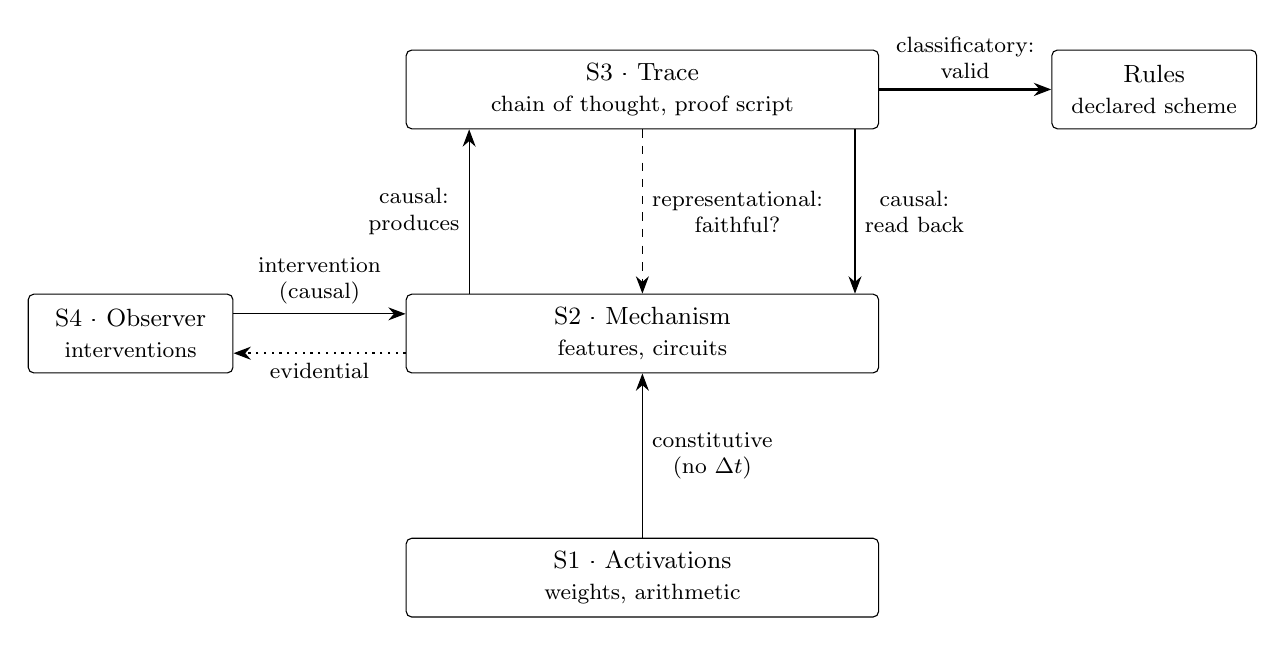
\begin{tikzpicture}[
    font=\small,
    box/.style={draw, rounded corners=2pt, align=center, minimum width=6.0cm,
                minimum height=1.0cm, inner sep=4pt},
    side/.style={draw, rounded corners=2pt, align=center, minimum width=2.6cm,
                minimum height=1.0cm, inner sep=4pt},
    lab/.style={font=\footnotesize, align=center},
    >={Stealth[length=2.2mm]}
  ]
  \node[box] (act)   at (0,0)    {S1 \textperiodcentered{} Activations\\\footnotesize weights, arithmetic};
  \node[box] (mech)  at (0,3.1)  {S2 \textperiodcentered{} Mechanism\\\footnotesize features, circuits};
  \node[box] (trace) at (0,6.2)  {S3 \textperiodcentered{} Trace\\\footnotesize chain of thought, proof script};
  \node[side] (rules) at (6.5,6.2) {Rules\\\footnotesize declared scheme};
  \node[side] (obs)   at (-6.5,3.1) {S4 \textperiodcentered{} Observer\\\footnotesize interventions};

  \draw[->] (act) -- node[lab, right] {constitutive\\(no $\Delta t$)} (mech);
  \draw[->] ([xshift=-22mm]mech.north) -- node[lab, left] {causal:\\produces} ([xshift=-22mm]trace.south);
  \draw[->, dashed] (trace.south) -- node[lab, right] {representational:\\faithful?} (mech.north);
  \draw[->] ([xshift=27mm]trace.south) -- node[lab, right] {causal:\\read back} ([xshift=27mm]mech.north);
  \draw[->, very thick] (trace) -- node[lab, above] {classificatory:\\valid} (rules);
  \draw[->] ([yshift=2.5mm]obs.east) -- node[lab, above] {intervention\\(causal)} ([yshift=2.5mm]mech.west);
  \draw[->, dotted, thick] ([yshift=-2.5mm]mech.west) -- node[lab, below] {evidential} ([yshift=-2.5mm]obs.east);
\end{tikzpicture}
\caption{One reasoning episode, with typed edges. A check of validity (thick) runs from
the trace to the rules. The edge that says whether the trace describes the mechanism
(dashed) runs from the trace to the mechanism. The same text is also read back as input
to later computation, a causal edge of its own. The observer intervenes, on the
mechanism as drawn or on the text that is read back; what comes back is evidence
(dotted).}
\label{fig:episode}
\end{figure}

None of the five is the real reasoning with the others as metaphors. Each is a legitimate
object with its own truth conditions. The difficulty arises only when a finding about one
is reported as a finding about another: when a valid proof is taken as evidence of how
the model computed, or a fluent chain of thought as a view of the mechanism.

\subsection{The trace is a representation}

A chain of thought is text the model writes. Its relation to the computation that
produced it is representational: the text describes a route to the answer. Like any
representation it can fail by misrepresenting. \citet{turpin2023} biased models toward
particular answers, for instance by making the correct option always ``(A)'' in the
examples, and found that the models followed the bias while their written explanations
did not mention it. \citet{chen2025} found the same pattern in models trained to reason
before answering: given a hint that changed their answer, they often did not say so in
their chain of thought.

Such findings are often reported with outcome labels: the model ``lied'' or
``rationalised''. Each label adds a claim about intent or mechanism that the observation
does not support. The observation is narrower: a representational edge failed. The text
describes one route; the computation took another. Naming the edge type names the
failure condition, correspondence, and with it what a test has to compare: the text
with the process that produced it.

The same text has a second role. Each written token is input to later forward passes,
so the trace is also a cause of later computation. The two roles are edges of different
types and can come apart: a text can influence the answer without describing how the
answer was reached, and it can describe without influencing. \citet{lanham2023} test the
causal role. They perturb the written reasoning, by truncating it or inserting
mistakes, and measure how far the final answer changes, and they find that the
dependence varies with model and task.

\subsection{What a proof kernel certifies}
\label{sec:kernel}

Now replace the chain of thought by a proof in Lean. The elaborator turns what the model
wrote into a proof term, and the kernel checks that term against the stated proposition,
in a declared environment of definitions and axioms. If the kernel accepts, the
proposition is proved relative to that environment, a guarantee no informal chain of
thought has. The edge that was checked is the classificatory edge from the trace to the
rules. The representational edge from the trace to the mechanism was not in view.

This can be stated exactly in a small model.

\begin{definition}[Reasoning system]
\label{def:rs}
A \emph{reasoning system} consists of a set $M$ of mechanisms, a set $T$ of traces, a
function $\produce : M \to T$, a predicate $\valid \subseteq T$ and a relation
$\faithful \subseteq T \times M$.
\end{definition}

\noindent
Here $\produce$ stands for the causal edge from mechanism to trace, $\valid$ for the
classificatory edge from trace to rules, and $\faithful(t,m)$ for the representational
edge: the trace $t$ describes the mechanism $m$. Write $F(m)$ for
$\faithful(\produce(m), m)$: the trace that $m$ writes describes $m$. A \emph{judgement
on traces} is a predicate $D \subseteq T$. It \emph{agrees with faithfulness} when, for
all $m \in M$, $D(\produce(m))$ holds if and only if $F(m)$.

\begin{proposition}[Validity is blind to the mechanism]
\label{prop:blind}
If $\produce(m_1) = \produce(m_2)$, then $\valid(\produce(m_1))$ if and only if
$\valid(\produce(m_2))$.
\end{proposition}

\begin{proposition}[When a judgement on traces can agree with faithfulness]
\label{prop:char}
A judgement on traces that agrees with faithfulness exists if and only if faithfulness
is constant among the mechanisms that write the same trace: for all $m_1, m_2 \in M$,
if $\produce(m_1) = \produce(m_2)$ then $F(m_1)$ if and only if $F(m_2)$.
\end{proposition}

\begin{corollary}[The obstruction]
\label{cor:split}
If two mechanisms write the same trace and the trace describes one of them and not the
other, that is, $\produce(m_1) = \produce(m_2)$, $F(m_1)$ and not $F(m_2)$, then no
judgement on traces agrees with faithfulness.
\end{corollary}

\noindent
These results need no assumption about the relation $\faithful$. They are checked in
Lean (Section~\ref{sec:mech}); the proofs take a few lines each. A judgement on traces
can be anything that looks only at the trace: a proof kernel, a reward model, a human
grader, a comparison with a reference answer. Suppose two routes, one following the
stated steps and one using an unmentioned hint, write the same valid text, and the text
describes the first and not the second. Then no judgement on the text sorts the
faithful episode from the unfaithful one. Appendix~\ref{app:uniqueness} gives one
condition under which a shared trace must have different verdicts, and the two-route
example from the package.

\begin{remark}[The results are elementary]
Proposition~\ref{prop:blind} is the congruence of equality.
Proposition~\ref{prop:char} says that a function of the trace can track a property of
mechanisms exactly when that property does not vary among the mechanisms behind one
trace. The paper claims no depth for these statements. Their use is that they fix which
edge a check tests, in a setting where one word lets a guarantee about one edge pass for
a guarantee about another.
\end{remark}

\begin{remark}[Scope]
\label{rem:scope}
(a) \emph{Existence, not computation.} A judgement on traces is an arbitrary predicate.
Proposition~\ref{prop:char} says when one exists that agrees with faithfulness, not
that it can be computed or found. In particular, a shared trace is by itself no
obstruction: if two mechanisms write the same trace and it describes neither, the
judgement that rejects the trace is right about both.
(b) \emph{Decision, not evidence.} The results do not say that a trace carries no
evidence about the mechanism. A feature of the text may correlate with faithfulness
across many episodes. What Corollary~\ref{cor:split} excludes is a judgement on the
text that is right on both episodes of a shared trace with different verdicts.
(c) \emph{Production as a function.} $\produce$ is a function for simplicity. The
argument uses only that one trace occurs with two mechanisms.
\end{remark}

Whether real models contain two computations that write an identical trace with
different verdicts is an empirical question that this paper does not answer. The
studies cited above show episodes in which the written reasoning omits a factor that
changed the answer. They motivate the distinction between validity and faithfulness.
They do not exhibit such a pair, and were not designed to.

\subsection{Two clocks: layers and tokens}

Within one forward pass, a computation can only be as serial as the network is deep: each
layer is one step, and the depth is fixed. A chain of thought adds a second sequence,
token positions. Every written token triggers a new forward pass that can read
everything before it, so the serial depth available grows with the length of the trace.
\citet{merrill2024} make this precise for a class of transformers. With logarithmically
many intermediate steps the gain is slight; with linearly many, under an architectural
assumption, all regular languages can be recognised; with polynomially many, the class
is exactly the problems solvable in polynomial time. Under standard
complexity-theoretic assumptions these are strict extensions of what the same
transformers compute without intermediate steps.

So the question of how many steps a model can reason has no answer until the sequence is
declared: layers or tokens. The two lie in different places in
Table~\ref{tab:reasoning}. Depth in layers is inside the mechanism (S2). Depth in tokens
runs through the trace (S3), because the intermediate results are written down and read
back. Approaches that feed continuous hidden states back in place of tokens, such as
that of \citet{hao2024}, keep the second sequence and remove the written layer. The
computation is no less real for that. It is less legible: the representation that could
at least be read, and sometimes checked, is gone.

\subsection{Grading the answer, grading the steps}

Training follows the same division. Outcome-based rewards grade only the final answer.
Process supervision grades each step, and on competition mathematics it trained more
reliable reward models than outcome supervision did \citep{lightman2023}. A graded step
is still a written step. Process supervision moves the judgement from the end of the
trace to its inside; it does not move it off the trace's layer, and
Proposition~\ref{prop:char} applies to it unchanged.

What goes beyond a judgement on a fixed text is an intervention, and there are two
places to intervene. One is the text as input: the written reasoning is perturbed and
the change in the answer observed, as in the study of \citet{lanham2023}. This needs no
access to the model's internals. The other is the mechanism: ablation and activation
patching, and attribution graphs that trace which internal features drive which,
validated by such interventions \citep{lindsey2025}. In both cases the observer
obtains, by an evidential edge, an observation of how the process behaves under a
change, and not only an observation of the text. These methods are costly and partial.
A claim that a trace is faithful is a claim about a representational edge. Where
faithfulness differs between computations that write the same trace, an exact judgement
needs information beyond the trace (Corollary~\ref{cor:split}), and interventions are
one way to obtain it.

\paragraph{What the field does, and what the rule adds.} Interpretability research
already separates faithfulness from plausibility and already tests explanations by
intervention; causal abstraction gives that practice a formal theory
(Section~\ref{sec:related}). The rule adds a plain statement of what follows for checks
on text. Validity is a classificatory edge from text to rules. Faithfulness is a
representational edge from text to mechanism. Whatever a check on the trace establishes,
it establishes about the trace, and a model's own account of how it reasoned is one more
trace. This does not make verified proofs less valuable: a valid proof is valid, whatever
produced it. It limits what else may be concluded from the check.

\section{Mechanisation in Lean 4}
\label{sec:mech}

The following parts of this paper are formalised in the Lean package \code{lem-lean}
\citep{kreinzlemlean}: the graph model of LEM on which the vocabulary rests, the typed
crossing of Definition~\ref{def:typed} with the two maps of
Section~\ref{sec:three-kinds} as worked examples, the small deontic model of
Section~\ref{sec:deontic}, and the model of reasoning systems of
Section~\ref{sec:kernel} with its results. Section~\ref{sec:mech-limits} says what is
not formalised. The listings in this section and in the appendix are taken unchanged
from version 0.4.0 of the package (commit \code{c111aaf}).

\subsection{Layers, nodes and typed edges}

The package follows the minimal formalisation given in LEM: a typed multigraph. Nodes are
indexed by layer, predicates are local to a layer, and edges form a type of their own
with a map to their edge type. Duration is a function on the causal edges alone. The
central definitions are these (the complete file is in
Appendix~\ref{app:basic}):

\lstinputlisting[linerange={32-36,45-48,70-88}]{code/Basic.lean}

\noindent
Three things follow from the types alone.

\begin{enumerate}[label=(\arabic*)]
  \item \emph{No cross-layer application of a predicate.} If a predicate is declared at
        one layer, applying it to a node of another layer is a type error. The layer is
        part of the node's type, so this holds even in a model whose two layers have the
        same carrier.
  \item \emph{No duration on a non-causal edge.} \code{CausalDuration.deltaT} takes a
        causal edge, which is an edge together with a proof that its type is causal. For
        a constitutive, classificatory or normative edge that proof does not exist, and
        a term that asks for its $\Dt$ is ill-typed.
  \item \emph{Duration belongs to the edge, not to the pair of nodes.} Because edges are
        a type of their own, two causal edges between the same two nodes are two edges
        and may carry different durations.
\end{enumerate}

\noindent
The first two are covered by negative tests: terms that Lean must reject, with the
expected error recorded. The third is a theorem.

\subsection{Typed crossings}
\label{sec:mech-crossing}

An edge of the graph above carries a label for its type and nothing else. A typed
crossing in the sense of Definition~\ref{def:typed} has two components, and the package
states the second as propositions that have to be proved:

\lstinputlisting[linerange={21-66}]{code/Crossing.lean}

\noindent
The structure \code{Crossing} itself holds only the kind and the relation. What the
crossing carries is not stored in it: each preservation statement is a separate theorem
about the crossing. The declared crossing together with its proved statements is what
Definition~\ref{def:typed} calls a typed crossing. \code{transport} is the reuse of a
claim. It takes the preservation proof as an
argument, so a claim established at the source cannot be asserted at the target without
one. \code{kind\_not\_determined} holds by construction: the kind is a field that the
relation does not constrain. The theorem records that design decision. It is not a
discovery about maps.

The two maps of Section~\ref{sec:three-kinds} are stated as crossings with declared
kinds. For the cast, addition is carried unconditionally, subtraction under its side
condition and not without it, and the order is invariant. The listing shows the
definition and the two results on subtraction; the rest is in
Appendix~\ref{app:crossing}.

\lstinputlisting[linerange={80-84,95-110}]{code/Crossing.lean}

\noindent
The reading of a 64-bit vector as a number is treated in the same way: addition is
carried while nothing overflows, and not otherwise. Both maps are proved injective, and their declared kinds differ. This is the
formal counterpart of the observation that two maps of the same structure can be used
in different roles.

\subsection{Reasoning traces}

The model of Section~\ref{sec:kernel} and its results are formalised as follows. The
proofs are included to show their size. Proposition~\ref{prop:blind} is
\code{valid\_blind\_to\_mechanism}, Proposition~\ref{prop:char} is
\code{trace\_only\_test\_iff} and Corollary~\ref{cor:split} is
\code{no\_trace\_only\_test\_of\_split}. In this file the reading of \code{produce},
\code{valid} and \code{faithful} as a causal, a classificatory and a representational
edge is given in comments. The types do not enforce it. The remaining results of the
file are in Appendix~\ref{app:uniqueness}.

\lstinputlisting[linerange={29-40,45-49,74-101}]{code/Trace.lean}

\subsection{What is checked}

Table~\ref{tab:mech} lists the content of the package. It has no dependency on Mathlib
and contains no \code{sorry}. Lean's \code{\#print axioms} reports at most
\code{propext}, one of Lean's three standard axioms; the results on reasoning traces,
the deontic results and the locality results use no axioms. The toolchain is pinned to
Lean~4.35.0, and the build, including the negative tests, runs in continuous
integration.

\begin{table}[t]
\centering\small
\begin{tabularx}{\textwidth}{@{}P{3.1cm}L@{}}
\toprule
File & Content \\
\midrule
\code{Basic.lean} &
  Layers, layer-indexed nodes, layer states, local predicates and relations, declared
  co-reference, the six edge types, the event graph, causal duration, the three deontic
  types, the type-level stratum. \\
\code{Duration.lean} &
  No duration for constitutive, classificatory or normative edges; the total,
  option-valued reading of $\Dt$ is undefined exactly on the non-causal edges; two
  parallel causal edges may carry different durations. \\
\code{Locality.lean} &
  A layer-respecting state assignment on the whole graph is the same thing as a family
  of layer states, and a predicate on the whole graph the same thing as a family of
  local predicates. \\
\code{Deontic.lean} &
  With three norm types the type alone settles the standing of an omission; with two it
  does not; the reduction of prohibition to obligation leaves every verdict on an
  omission unchanged (Section~\ref{sec:deontic}; statements in
  Appendix~\ref{app:deontic}). \\
\code{Crossing.lean} &
  A crossing with a declared kind; preservation, reflection and invariance of
  predicates; invariance of a relation; an operation carried under a side condition;
  reuse of a claim by a preservation proof. Two worked crossings, $\N \to \Z$ and
  \code{BitVec 64} $\to \N$, with their side conditions and counterexamples. \\
\code{Trace.lean} &
  Propositions~\ref{prop:blind} and~\ref{prop:char} and Corollary~\ref{cor:split}; the
  uniqueness-based results and the two-route example of
  Appendix~\ref{app:uniqueness}. \\
\code{Rejections.lean} &
  Negative tests: a predicate of one layer applied to a node of another, also where
  both layers share a carrier; $\Dt$ asked of a normative edge. \\
\bottomrule
\end{tabularx}
\caption{Content of the \code{lem-lean} package, version 0.4.0.}
\label{tab:mech}
\end{table}

\subsection{What the mechanisation does and does not establish}
\label{sec:mech-limits}

\paragraph{It is partial.} Of the three cases, only the first is stated as a typed
crossing in Lean, and for two maps and a handful of operations. The package does not
reproduce what Mathlib's bundled morphisms and cast lemmas provide, and it does not
connect to them. The refinement case of Section~\ref{sec:refinement} is not formalised
at all. The reasoning-system model of Section~\ref{sec:kernel} is formalised on its own
terms and not as an instance of the crossing structure. The event graph and the
crossing structure are also not connected: an edge of the graph does not carry
preservation statements.

\paragraph{It checks consequences, not fit.} The checker establishes that the stated
results follow from the stated definitions, and that a declaration, once made, is used
consistently. It does not establish that the definitions fit any real system, or that a
declared type is the right one. The encoding does not decide the type of any edge: types
are declared by the modeller. The tests by which LEM proposes to decide them are not
formalised, and LEM records that they have not been validated between raters.

The same holds for the model of reasoning systems. That the results of
Section~\ref{sec:kernel} are machine-checked says nothing about whether
Definition~\ref{def:rs} describes a given model well. That is a question about the
crossing from the formal model to the system modelled, a representational one, and the
kernel does not test it. The paper's thesis applies to its own artefact: verifying the
proofs verifies the proofs.

\section{Related work}
\label{sec:related}

\subsection{Coercions and subtyping}

Implicit coercions have a long theory. \citet{breazu1991} interpret inheritance as
implicit coercion and prove \emph{coherence}: the meaning of a term does not depend on
which typing derivation, and so which insertion of coercions, is chosen.
\citet{luo1999} develops coercive subtyping for dependent type theories, in which
coercions are an abbreviation mechanism and coherence, the uniqueness of the coercion
between two types, is the central requirement. Coherence answers the question
\emph{which} map is inserted. The question raised in Section~\ref{sec:casts} is the next
one: given the map, \emph{what} it preserves. The two are independent, since the unique
cast from $\N$ to $\Z$ still fails to commute with truncated subtraction.

Within Lean, the simplification of casts is described by \citet{lewis2020}, whose
classification of lemmas into move, elim and squash is used in
Section~\ref{sec:casts}, and the design of bundled morphisms and their classes by
\citet{baanen2022}. This paper adds nothing to that machinery. It reads it as an
instance of a more general practice.

The requirement that truth be invariant under a change of notation is the satisfaction
condition of the theory of institutions \citep{goguen1992}, where it is an axiom on
translations between signatures. Predicate locality asks for the same invariance, but as
an obligation to be discharged for each predicate that is reused across a boundary, and
with the expectation that it will sometimes fail.

\subsection{Refinement and the preservation of properties}

That refinement preserves properties of single traces and not, in general, properties of
sets of traces is the subject of \citet{clarkson2010}; the distinction between safety and
liveness on which Section~\ref{sec:deontic} relies is due to \citet{alpern1985}. The
theory of secure compilation makes the preservation list explicit. \citet{abate2019}
define a family of criteria for compilers according to the class of properties that is
preserved against adversarial contexts (trace properties, safety properties,
hyperproperties and relational hyperproperties) and establish how the criteria relate;
\citet{patrignani2019} survey the earlier criterion of full abstraction. These criteria
are the most developed existing counterpart of the second component of a typed crossing:
they type a compiler by what it preserves.

The present paper is less precise than that work and differs in scope. It adds the first
component, the kind of the crossing, and it includes among the things a crossing may fail
to carry some that are not properties of traces at all: duration
(Section~\ref{sec:duration}), provenance, and the standing of a step under a norm.

\subsection{Faithfulness, causal abstraction and monitoring}

\citet{jacovi2020} separate the faithfulness of an explanation from its plausibility and
argue for a graded notion of faithfulness in place of a binary one. The model in
Section~\ref{sec:kernel} uses a binary relation, which is the simplest setting in which
the point about checks on text can be made; a graded notion would need a different
formal treatment. Empirical work on written reasoning includes \citet{turpin2023},
\citet{lanham2023} and \citet{chen2025}. \citet{barez2025} argue from this evidence that
a chain of thought should not be treated as an explanation without causal validation,
which is the conclusion of Section~\ref{sec:reasoning} reached from the empirical side.

The formal theory of the crossing between an explanation and a mechanism is causal
abstraction \citep{geiger2025}: a high-level causal model is an abstraction of a
low-level one when interventions on the two correspond, and this is tested by
intervening on the network. Proposition~\ref{prop:char} is far weaker than that theory
and compatible with it. Its one point is conditional: where faithfulness differs
between mechanisms that produce the same description, an exact judgement requires
information beyond the description. Interventions on the network, as used in causal
abstraction, are one way to obtain such information.

\citet{korbak2025} argue that written reasoning is nevertheless a valuable signal for
monitoring models, and a fragile one, since training methods or architectures may make
it less legible. That position is consistent with this paper. A monitor that reads a
trace obtains evidence, by an evidential edge, about what the model may do. The results
here concern a different question, whether a check on the trace can decide that the
trace describes the computation, and Remark~\ref{rem:scope}(b) keeps the two apart.

\subsection{Levels and edge types}

The distinction between constitutive and causal relations between levels is taken from
the mechanistic account of \citet{craver2007}, and the intervention test for causal
edges from \citet{woodward2003}. The edge taxonomy, the five structures and the axioms
are those of LEM \citep{kreinzlem}, which discusses its own relation to the literature
on levels, ontology and risk modelling.

\section{Limitations and predictions}
\label{sec:limits}

\subsection{Limitations}

\paragraph{Three cases, chosen by the author.} The cases were selected because the
vocabulary fits them. They are evidence that the vocabulary of LEM can be carried to
these three settings, and no more. Cases in which typing a crossing adds nothing, or in
which the kinds proposed here do not apply, were not searched for.

\paragraph{A parallel, not an identity.} The three roles of a map in
Section~\ref{sec:three-kinds} and the six edge types of Table~\ref{tab:edges} overlap but
were arrived at separately. The paper does not give one classification that covers both,
and does not claim that either list is complete or that its members exclude one
another.

\paragraph{The mechanisation is partial.} The Lean package states the typed crossing
and works it out for two maps from the first case. The refinement case is not
formalised, the reasoning-system model is not expressed as a crossing, and the package
is not connected to Mathlib (Section~\ref{sec:mech-limits}). That the kind of a
crossing is not determined by its relation holds in the formal model by construction,
and so adds no evidence for the claim.

\paragraph{The kind is declared, not decided.} The rule asks that the kind of a crossing
be declared. It does not supply a procedure that decides it. LEM proposes tests for edge
types, two of which are used in Section~\ref{sec:duration}; they are not formalised, and
their agreement between independent raters has not been measured. Where two modellers
would declare different kinds for one crossing, the rule exposes the disagreement and
does not resolve it.

\paragraph{The results are elementary and rest on a model.} The weight of
Section~\ref{sec:kernel} is carried by Definition~\ref{def:rs}, not by the proofs. The
model treats faithfulness as a binary relation between a trace and a mechanism,
presupposes that mechanisms can be individuated, and takes production to be a function.
Each is a simplification (Remark~\ref{rem:scope}), and a graded notion of faithfulness
is not covered. The deontic model of Section~\ref{sec:deontic} is smaller still: it has
no deadlines and no conditions of applicability.

\paragraph{No empirical evaluation.} The paper reports no experiments. In particular it
does not show that real models contain two computations that write the same trace with
different verdicts, nor how often, which is what determines how much
Corollary~\ref{cor:split} matters in practice.

\paragraph{The source of the vocabulary.} LEM is a method proposal by the same author,
developed for risk modelling and published as a preprint. Its own validation is open,
and this paper inherits that status for everything it takes from LEM.

\paragraph{An outside view.} The paper addresses three research communities, and the
author's own field is risk modelling. The accounts given here of Mathlib, of
verification practice and of interpretability research rest on the literature cited, not
on work inside those communities. Corrections from them are invited.

\subsection{Two predictions}

The argument yields two predictions that existing benchmarks of automated theorem
proving could test. They are independent, and the second is the one that bears on the
rule.

\begin{prediction}[Crossings are where provers fail]
Among the failures of automated provers on formal proof tasks, proof steps that cross a
boundary (a cast, a change of representation, a step from an operational semantics to an
invariant) are over-represented, relative to their share of all steps and compared with
steps inside one structure.
\end{prediction}

\begin{prediction}[Declaring the kind helps beyond supplying the lemmas]
Give a prover the preservation lemmas that are relevant to the crossings in a task. A
prover that is given, in addition, a declaration of the kind of each crossing fails
less often at crossings than one that is given the same lemmas without it.
\end{prediction}

No measurement is cited or reported here. The first prediction requires a classification
of proof steps into crossing and non-crossing ones, fixed before the failure data are
examined, and would be refuted by a failure rate at crossings that does not differ from
the rate elsewhere. The second needs the baseline it names. Without it, an improvement
would show only that supplying useful lemmas helps a prover, which is not in doubt. If
the declaration of kind adds nothing over the lemmas, the first component of
Definition~\ref{def:typed} has no measurable use in this setting, and the paper's case
for it would rest on the diagnostic uses of Sections~\ref{sec:refinement}
and~\ref{sec:reasoning} alone.

\section{Conclusion}
\label{sec:conclusion}

A cast, a simulation relation and the link from a written trace to the computation
behind it have one thing in common. Each carries a claim from one structure into
another, and none of them, as usually written, says what kind of crossing it is or what
survives it. The fields that depend on these crossings have each found ways to say it
locally: lemmas registered for a cast, a preservation proof for each further property,
interventions on a model to test what its text says about it.

The proposal of this paper is modest in its means. A crossing along which claims are
carried becomes an object with a type: its kind, what it preserves, and under which
conditions. What was carried by an overloaded symbol, by the word ``verified'' or by the
word ``reasoning'' becomes something that can be inspected and checked. For written
model reasoning this gives a statement that is exact within its assumptions. Validity is
one crossing and faithfulness another, and where one trace is written by two
computations and describes only one of them, no check on the trace tells them apart.
Verify the trace, and you have verified the trace.

\section*{Declarations}
\addcontentsline{toc}{section}{Declarations}

\paragraph{Artefact availability.} The Lean package \code{lem-lean} is available at
\url{https://github.com/Barnes70/lem-lean} under the Apache License~2.0. This paper
refers to version 0.4.0 (tag \code{v0.4.0}, commit \code{c111aaf}), which builds with
Lean~4.35.0. The build command is
\code{lake build}, and the negative tests are run with the command
\code{lake env lean test/Rejections.lean}.

\paragraph{Prior publication.} Parts of this paper draw on two essays by the author,
\emph{Invisible Coercions and Untyped Refinement} and \emph{Where Does a Model Reason?},
published at \url{https://www.barnes.ch} in 2026.

\paragraph{Use of AI assistance.} The author used AI language models as assistants: for
drafting and revising the text, for checking references and for developing the Lean
code (Claude, Anthropic), and for critical review of drafts. All Lean code is checked
by the Lean kernel. The author has reviewed the content and is responsible for it.

\paragraph{Competing interests.} The author is the originator of Layered Event Modelling
and of the TLCTC framework, both of which this paper cites. The author declares no other
competing interests.

\paragraph{Funding.} This work received no external funding.

\paragraph{Licence.} The text and figures of this paper are licensed under Creative
Commons Attribution~4.0 International (CC~BY~4.0). The Lean code is licensed under the
Apache License~2.0.


\newcommand{\doi}[1]{doi: \href{https://doi.org/#1}{\nolinkurl{#1}}}
\bibliographystyle{plainnat}
\bibliography{refs}

\appendix
\section{The typed multigraph in Lean 4}
\label{app:basic}

The complete definitions of \code{LemLean/Basic.lean}. Section references in the
comments are to LEM \citep{kreinzlem}.

\lstinputlisting[linerange={17-105}]{code/Basic.lean}

\section{The deontic results}
\label{app:deontic}

From \code{LemLean/Deontic.lean}: the standing of an omission under three norm types and
under two, and the three results of Section~\ref{sec:deontic}. The code calls the
omission an idle step and writes it \code{skip}; it means that the agent does not
perform the act, not a stuttering step of a refinement. The model has no deadline and no
condition of applicability, so an obligation in it is one that is applicable, due and
undischarged.

\lstinputlisting[linerange={20-50,53-104}]{code/Deontic.lean}

\section{The two worked crossings}
\label{app:crossing}

From \code{LemLean/Crossing.lean}: the three roles, the cast from the natural numbers to
the integers, and the reading of a 64-bit vector as a number.

\lstinputlisting[linerange={70-162}]{code/Crossing.lean}

\section{A condition under which a shared trace has different verdicts}
\label{app:uniqueness}

Corollary~\ref{cor:split} needs two mechanisms that write the same trace with different
verdicts. One condition that forces different verdicts is that a trace describes at
most one mechanism.

\begin{assumption}[A trace describes at most one mechanism]
\label{ass:functional}
For all $t \in T$ and $m_1, m_2 \in M$: if $\faithful(t,m_1)$ and $\faithful(t,m_2)$ then
$m_1 = m_2$.
\end{assumption}

\begin{proposition}[A shared trace is not faithful to both]
\label{prop:both}
Under Assumption~\ref{ass:functional}, if $m_1 \neq m_2$ and
$\produce(m_1) = \produce(m_2)$, then not both $F(m_1)$ and $F(m_2)$.
\end{proposition}

\begin{corollary}
\label{cor:functional}
Under Assumption~\ref{ass:functional}, if $m_1 \neq m_2$,
$\produce(m_1) = \produce(m_2)$ and $F(m_1)$, then no judgement on traces agrees with
faithfulness.
\end{corollary}

The assumption is contestable: a useful description can fit several implementations.
One response is to count mechanisms that differ only in ways the description is not
meant to capture as one element of $M$. That requires $\produce$ to be well defined on
the resulting classes, which can fail, since mechanisms that are alike in the relevant
respect may still write different text. Proposition~\ref{prop:char} and
Corollary~\ref{cor:split} do not use the assumption and avoid the question.

In the Lean file, Proposition~\ref{prop:both} is the theorem
\code{not\_both\_faithful}, and the corollary is the theorem
\code{no\_trace\_only\_faithfulness\_test}. The file ends with a two-route example, in
which one valid trace is written by a route that follows the stated rules and by a
route that uses a hint the trace does not mention. It shows that the hypotheses can be
satisfied together.

\lstinputlisting[linerange={41-44,50-72,105-142}]{code/Trace.lean}


\end{document}
